%%%%%%%%%%%%%%%%%%%%%%%%%%%%%%%%%%%%%%%%%%%%%%%%%%%%%%
% Flink Stateful Streaming Presentation               %
% Based on: How Flink Handles Stateful Streaming      %
%           at Large Scale                             %
%%%%%%%%%%%%%%%%%%%%%%%%%%%%%%%%%%%%%%%%%%%%%%%%%%%%%%

\documentclass[aspectratio=169]{beamer}
\usepackage{hyperref}
\usepackage[T1]{fontenc}

% other packages
\usepackage{latexsym,amsmath,amssymb,xcolor,multicol,booktabs,calligra}
\usepackage{graphicx,listings,stackengine}
% SVGs pre-converted to PDF via rsvg-convert

\author{Xuan-Cuong Le}
\title[Flink Stateful Streaming]{How Flink Handles Stateful Streaming at Large Scale}
\subtitle{From Kafka Message to Exactly-Once Delivery}
\institute{cuongkane.com}
\date{\today}
\usepackage{UTU}

% defs
\def\cmd#1{\texttt{\color{red}\footnotesize $\backslash$#1}}
\def\env#1{\texttt{\color{blue}\footnotesize #1}}
\definecolor{utu_green}{RGB}{173,203,0}
\definecolor{utu_blue}{RGB}{93,155,162}
\definecolor{utu_pink}{RGB}{248,72,94}
\definecolor{halfgray}{gray}{0.55}
\definecolor{lightgray}{gray}{0.9}

\lstset{
    basicstyle=\ttfamily\small,
    keywordstyle=\bfseries\color{utu_green},
    emphstyle=\ttfamily\color{utu_blue},
    stringstyle=\color{utu_pink},
    numbers=left,
    numberstyle=\small\color{halfgray},
    rulesepcolor=\color{red!20!green!20!blue!20},
}


\begin{document}

\begin{frame}
    {\small
    \titlepage
    }
\end{frame}

% ============================================================
\section{Stateful Stream Processing}
% ============================================================

\begin{frame}{What Is Stateful Stream Processing?}
    Most stream processing is \textbf{stateless}: message in, transform, push out.

    \vspace{0.3cm}
    But many real-world problems require \textbf{remembering things across messages}:
    \begin{itemize}
        \item \textbf{Deduplication} -- ``Have I seen this event ID before?''
        \item \textbf{Windowed aggregations} -- ``How many orders in the last 5 minutes?''
        \item \textbf{Pattern detection} -- ``Alert if a user fails login 3 times in a row''
    \end{itemize}

    \vspace{0.3cm}
    \colorbox{utu_green!20}{\parbox{0.9\textwidth}{
        \centering
        The moment your processor needs to remember something between messages, you have \textbf{stateful} stream processing.
    }}
\end{frame}

\begin{frame}{The Naive Approach: External State Store}
    A Kafka consumer that checks PostgreSQL/Redis for every message.

    \vspace{0.3cm}
    \textbf{This works at moderate scale.} For thousands -- even tens of thousands -- of messages/second, an external store is perfectly fine.

    \vspace{0.3cm}
    \begin{center}
        \textbf{The question is what happens when you outgrow it.}
    \end{center}
\end{frame}

\begin{frame}{Why External Stores Break Down at Scale}
    \begin{itemize}
        \item \textbf{Network round-trips kill throughput}
        \begin{itemize}
            \item At 1M msg/s across 8 partitions: 2M round-trips/second to Redis
            \item Each round-trip adds 0.5--2ms latency
            \item Pipeline bottleneck becomes the network, not the computation
        \end{itemize}

        \vspace{0.2cm}
        \item \textbf{Consistency is painful}
        \begin{itemize}
            \item Crash between Redis write and Kafka produce $\rightarrow$ inconsistent state
            \item Exactly-once across two systems requires distributed transactions
        \end{itemize}

        \vspace{0.2cm}
        \item \textbf{Scaling state independently from compute is wasteful}
        \begin{itemize}
            \item Redis cluster scales on state size, consumers on throughput
            \item Coupled in practice, managed separately
        \end{itemize}
    \end{itemize}

    \vspace{0.2cm}
    \colorbox{utu_pink!20}{\parbox{0.9\textwidth}{
        \centering
        External state turns \textbf{every message} into a distributed system problem.
    }}
\end{frame}

% ============================================================
\section{How Flink Solves This}
% ============================================================

\begin{frame}{Flink's Approach: Co-located State}
    \textbf{State lives inside the stream processor.}

    \vspace{0.3cm}
    \begin{itemize}
        \item Each parallel operator instance has its own \textbf{local RocksDB} store
        \item No network round-trips for state access
        \item Local disk reads that hit an in-memory cache 95\%+ of the time
    \end{itemize}

    \vspace{0.3cm}
    But co-located state introduces new problems:
    \begin{itemize}
        \item How do you make local state \textbf{durable}?
        \item How do you \textbf{recover} it after a crash?
        \item How do you \textbf{redistribute} it when you scale up?
    \end{itemize}

    \vspace{0.2cm}
    \colorbox{utu_blue!20}{\parbox{0.9\textwidth}{
        \centering
        Flink's answer: checkpoint barriers, incremental snapshots, and two-phase commits.
    }}
\end{frame}

\begin{frame}{The Pipeline We'll Trace}
    \begin{figure}[htpb]
        \centering
        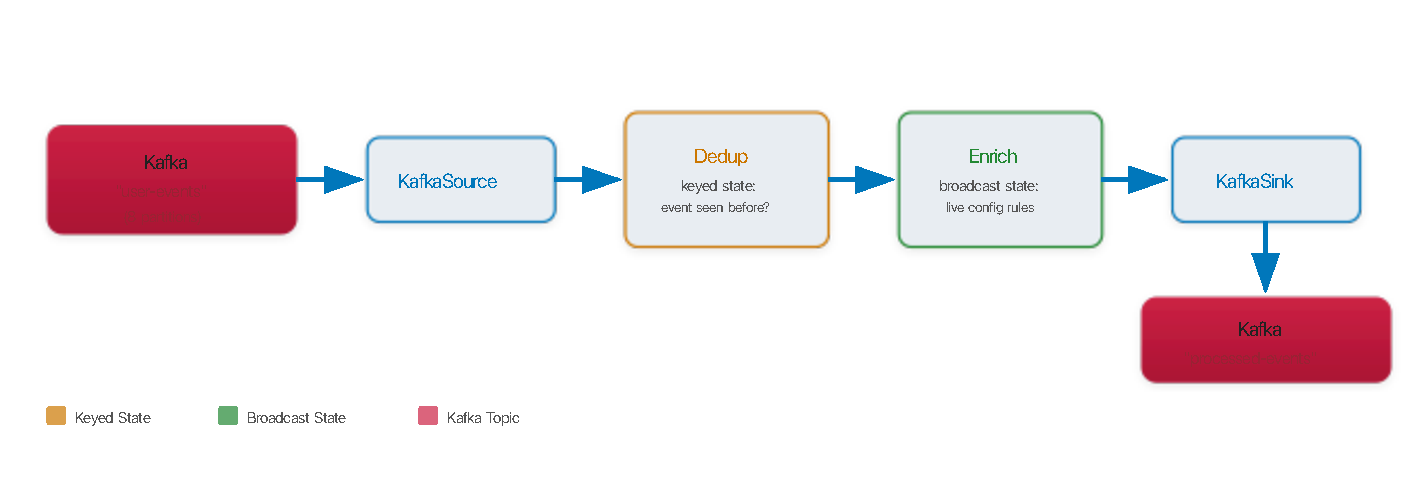
\includegraphics[width=0.85\textwidth]{fig/pipeline_flow.pdf}
        \caption{A single Kafka message through: Source $\rightarrow$ Dedup $\rightarrow$ Enrich $\rightarrow$ Sink}
    \end{figure}
\end{frame}

% ============================================================
\section{Flink Architecture}
% ============================================================

\begin{frame}{Flink's Moving Parts}
    \begin{columns}[T]
        \begin{column}{0.48\textwidth}
            \textbf{JobManager} -- The brain
            \begin{itemize}
                \item Coordinates the entire job
                \item Triggers checkpoints, handles failures
                \item Contains: Dispatcher, ResourceManager, JobMaster
            \end{itemize}

            \vspace{0.2cm}
            \textbf{TaskManager} -- The workers
            \begin{itemize}
                \item Separate JVM process (one K8s Pod)
                \item Registers with JobManager
                \item Offers computational capacity
            \end{itemize}
        \end{column}
        \begin{column}{0.48\textwidth}
            \textbf{Slot} -- Resource container
            \begin{itemize}
                \item Logical slice of TaskManager resources
                \item Hard-partitioned memory budget
            \end{itemize}

            \vspace{0.2cm}
            \textbf{Operator} -- Processing step
            \begin{itemize}
                \item KafkaSource, Dedup, Enrich, KafkaSink
                \item Defines \textit{what} to do with data
            \end{itemize}

            \vspace{0.2cm}
            \textbf{Subtask} -- Parallel instance
            \begin{itemize}
                \item Dedup with parallelism=8 $\rightarrow$ 8 subtasks
                \item A Java thread that processes data
            \end{itemize}
        \end{column}
    \end{columns}
\end{frame}

\begin{frame}{Hierarchy on One Machine}
    \begin{figure}[htpb]
        \centering
        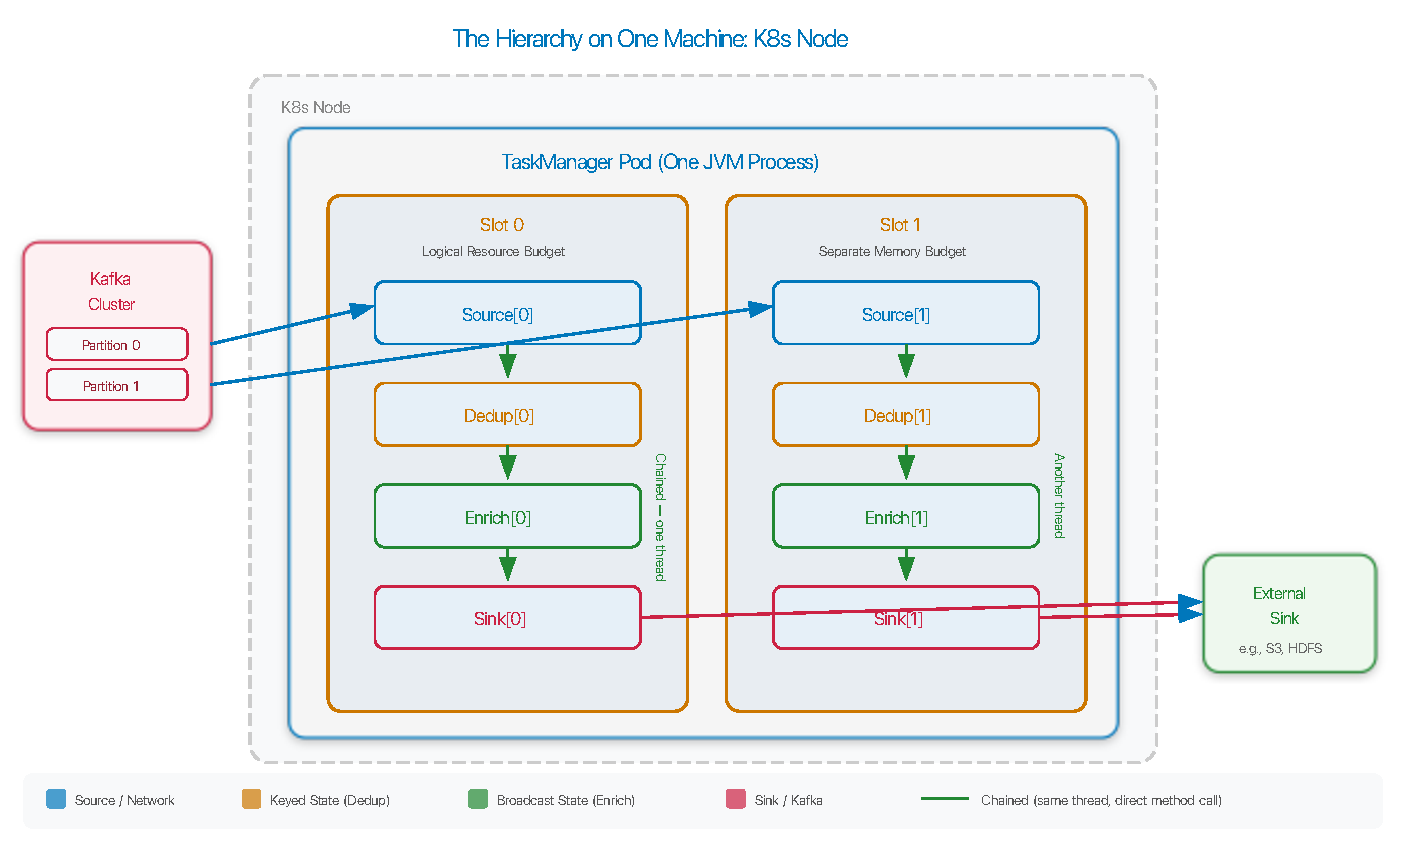
\includegraphics[keepaspectratio, height=0.8\textheight]{fig/single_node.pdf}
    \end{figure}
\end{frame}

\begin{frame}{Flink on Kubernetes (parallelism=8, 2 slots/TM)}
    \begin{figure}[htpb]
        \centering
        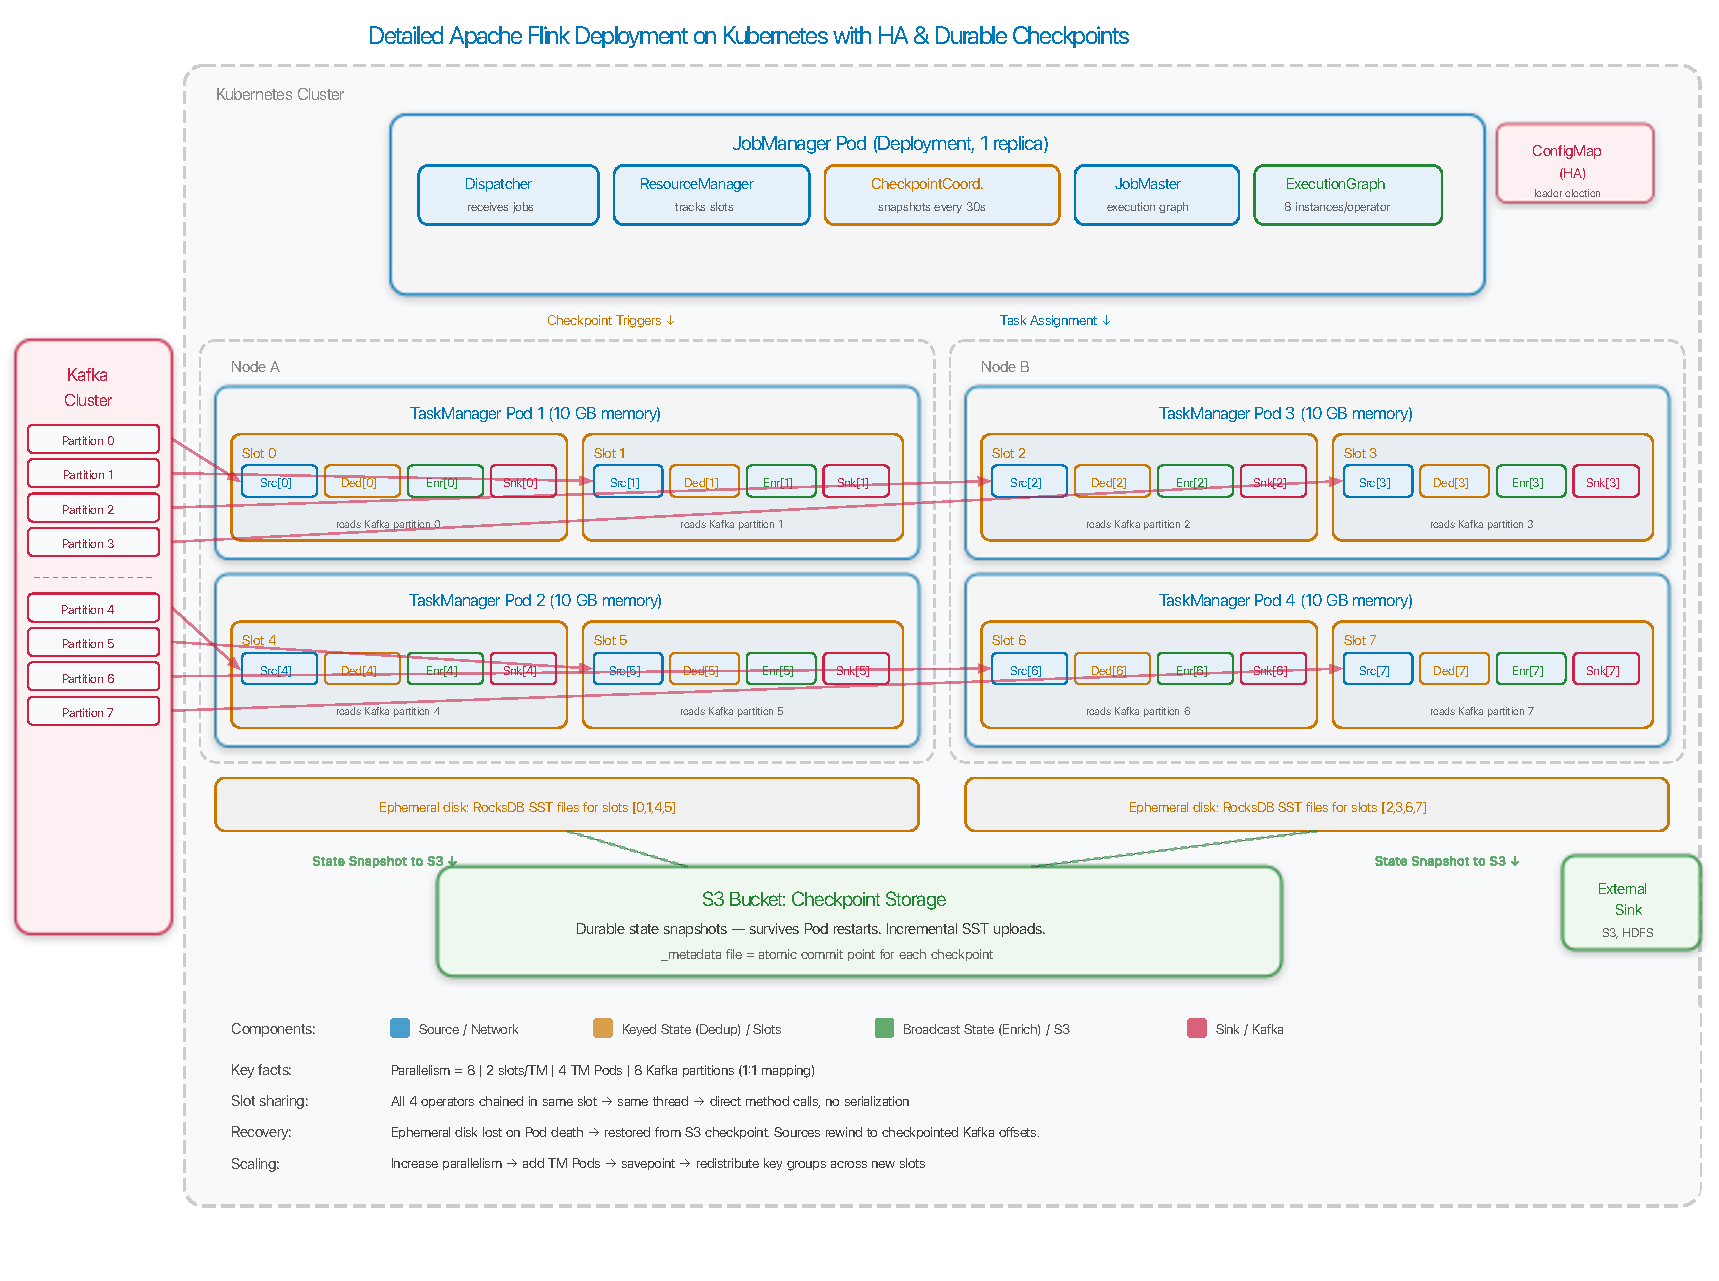
\includegraphics[keepaspectratio, height=0.8\textheight]{fig/flink_architect.pdf}
    \end{figure}
\end{frame}

\begin{frame}{Key Observations}
    \begin{itemize}
        \item \textbf{Each TaskManager Pod is one JVM process}
        \begin{itemize}
            \item 2 slots share the JVM heap but each gets \textbf{isolated managed memory}
        \end{itemize}

        \vspace{0.15cm}
        \item \textbf{8 Kafka partitions, parallelism 8, 8 slots} -- ideal 1:1 mapping
        \begin{itemize}
            \item Flink never splits one Kafka partition across multiple readers
        \end{itemize}

        \vspace{0.15cm}
        \item \textbf{Slot sharing}: all 4 operators run in the \textbf{same slot} for the same subtask index
        \begin{itemize}
            \item Chained into a single Java thread; data flows via direct method calls
        \end{itemize}

        \vspace{0.15cm}
        \item \textbf{RocksDB state on ephemeral disk} -- disappears when Pod dies
        \begin{itemize}
            \item Checkpoint data on S3 (durable); new Pods rebuild from S3
        \end{itemize}

        \vspace{0.15cm}
        \item \textbf{Scaling up} = more TM Pods + savepoint to redistribute state
    \end{itemize}
\end{frame}

% ============================================================
% Message Ingestion
% ============================================================

\begin{frame}[fragile]{Chapter 1: A Message Is Born}
    A user event arrives in Kafka \textbf{partition 3, offset 50701}:

    \vspace{0.3cm}
    \begin{center}
    \begin{lstlisting}[language=Java,basicstyle=\ttfamily\footnotesize]
{
  "event_id": "evt-88821",
  "user_id": "user-42",
  "action": "purchase",
  "amount": 59.99,
  "timestamp": 1712100000000
}
    \end{lstlisting}
    \end{center}
\end{frame}

\begin{frame}{Chapter 2: Flink Picks It Up}
    \textbf{Source[3]} -- the 4th parallel instance of KafkaSource, running in \textbf{Slot 3, TaskManager Pod 2, Node A}.

    \vspace{0.3cm}
    \begin{enumerate}
        \item Background fetcher thread calls Kafka's \texttt{poll()}
        \item Message arrives in a batch; placed into a hand-over queue
        \item Slot's task thread picks it up
        \item Source deserializes raw bytes into a Flink \texttt{StreamRecord}
    \end{enumerate}

    \vspace{0.3cm}
    \colorbox{utu_pink!20}{\parbox{0.9\textwidth}{
        \centering
        Flink does \textbf{NOT} use Kafka consumer group offsets for recovery. It stores offsets in its own checkpoint state.
    }}
\end{frame}

\begin{frame}{Stream Markers: Watermarks \& Checkpoint Barriers}
    \begin{figure}[htpb]
        \centering
        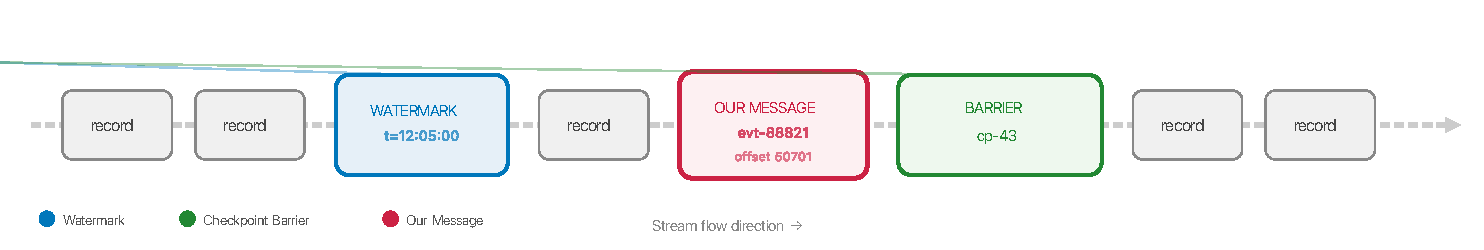
\includegraphics[width=0.85\textwidth]{fig/stream_markers.pdf}
    \end{figure}
\end{frame}

\begin{frame}{Watermarks -- ``When Can We Close a Time Window?''}
    \begin{itemize}
        \item A timestamp that flows through the stream meaning: \textbf{``all events before this value have already arrived''}
        \item Each \textbf{source subtask} generates watermarks based on event timestamps
        \item Each \textbf{subtask} tracks watermarks from all input channels
        \item Takes the \textbf{minimum} across all inputs
    \end{itemize}

    \vspace{0.3cm}
    \colorbox{utu_blue!20}{\parbox{0.9\textwidth}{
        \centering
        One straggling Kafka partition holds back \textbf{all} downstream time-based operations.
    }}
\end{frame}

\begin{frame}{Checkpoint Barriers -- ``Take a Snapshot at This Exact Point''}
    \begin{itemize}
        \item \textbf{JobManager's CheckpointCoordinator} sends ``start checkpoint 44'' to all sources
        \item Each \textbf{source subtask} injects a barrier into its output stream
        \item Barrier divides the stream: before $\rightarrow$ checkpoint 44, after $\rightarrow$ checkpoint 45
        \item Each \textbf{subtask} handles barrier alignment independently
    \end{itemize}

    \vspace{0.2cm}
    \begin{columns}[T]
        \begin{column}{0.48\textwidth}
            \textbf{Aligned mode} (default)
            \begin{itemize}
                \item Blocks fast channels
                \item Processes only slow ones
            \end{itemize}
        \end{column}
        \begin{column}{0.48\textwidth}
            \textbf{Unaligned mode} (opt-in)
            \begin{itemize}
                \item Continues all channels
                \item Includes in-flight records in checkpoint
                \item Avoids backpressure; larger checkpoints
            \end{itemize}
        \end{column}
    \end{columns}
\end{frame}

% ============================================================
% The Dedup -- Network Shuffle
% ============================================================

\begin{frame}{Chapter 3: Does This Message Need a Network Hop?}
    Dedup is keyed by \texttt{event\_id}. After \texttt{keyBy()}, Flink routes each record to the subtask that \textbf{owns} that key's state.

    \vspace{0.3cm}
    \begin{figure}[htpb]
        \centering
        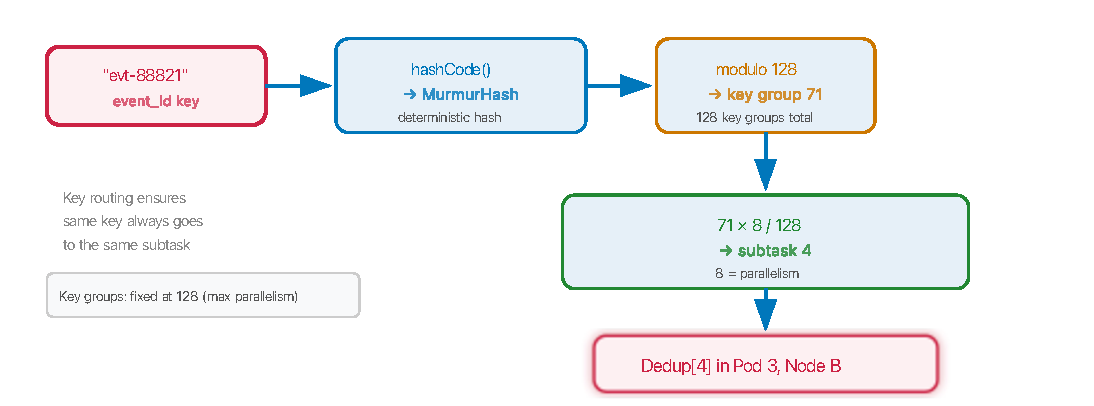
\includegraphics[width=0.8\textwidth]{fig/key_hashing.pdf}
        \caption{Key hashing: event\_id $\rightarrow$ hash $\rightarrow$ key group $\rightarrow$ subtask}
    \end{figure}
\end{frame}

\begin{frame}{What Happens on the Wire}
    Source[3] in Pod 2 (Node A) $\rightarrow$ \textbf{Dedup[4] in Pod 3 (Node B)}

    \vspace{0.3cm}
    \begin{enumerate}
        \item \textbf{Serialization}: message $\rightarrow$ bytes in a 32 KB network buffer
        \item \textbf{Partitioning}: \texttt{ResultPartition} has 8 sub-partitions; ours goes to sub-partition 4
        \item \textbf{TCP transport}: Netty over TCP, through K8s network (CNI plugin)
        \item \textbf{Deserialization}: Dedup[4]'s input gate $\rightarrow$ \texttt{StreamRecord} $\rightarrow$ Dedup operator
    \end{enumerate}

    \vspace{0.3cm}
    \textbf{Backpressure}: If Dedup[4] is slow $\rightarrow$ input buffers fill $\rightarrow$ no credits sent $\rightarrow$ sender blocks $\rightarrow$ Source[3] slows Kafka \texttt{poll()} rate. \textbf{No data is ever dropped.}
\end{frame}

% ============================================================
% State -- RAM or Disk?
% ============================================================

\begin{frame}{TaskManager Memory Layout}
    \begin{figure}[htpb]
        \centering
        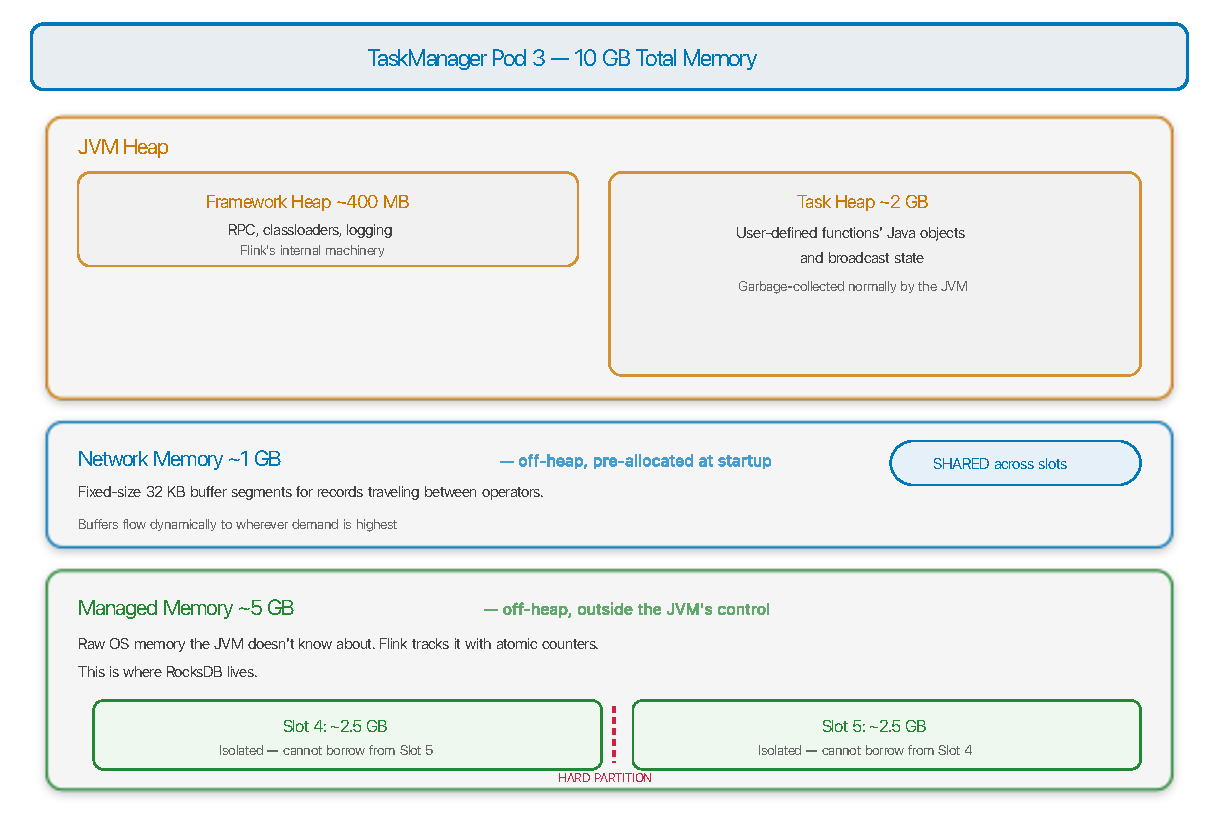
\includegraphics[keepaspectratio, height=0.75\textheight]{fig/tm_memory_layout.pdf}
    \end{figure}

    {\small Managed memory is \textbf{hard-partitioned per slot}. Slot 4 cannot steal from Slot 5.}
\end{frame}

\begin{frame}{Slot Memory Breakdown}
    \begin{figure}[htpb]
        \centering
        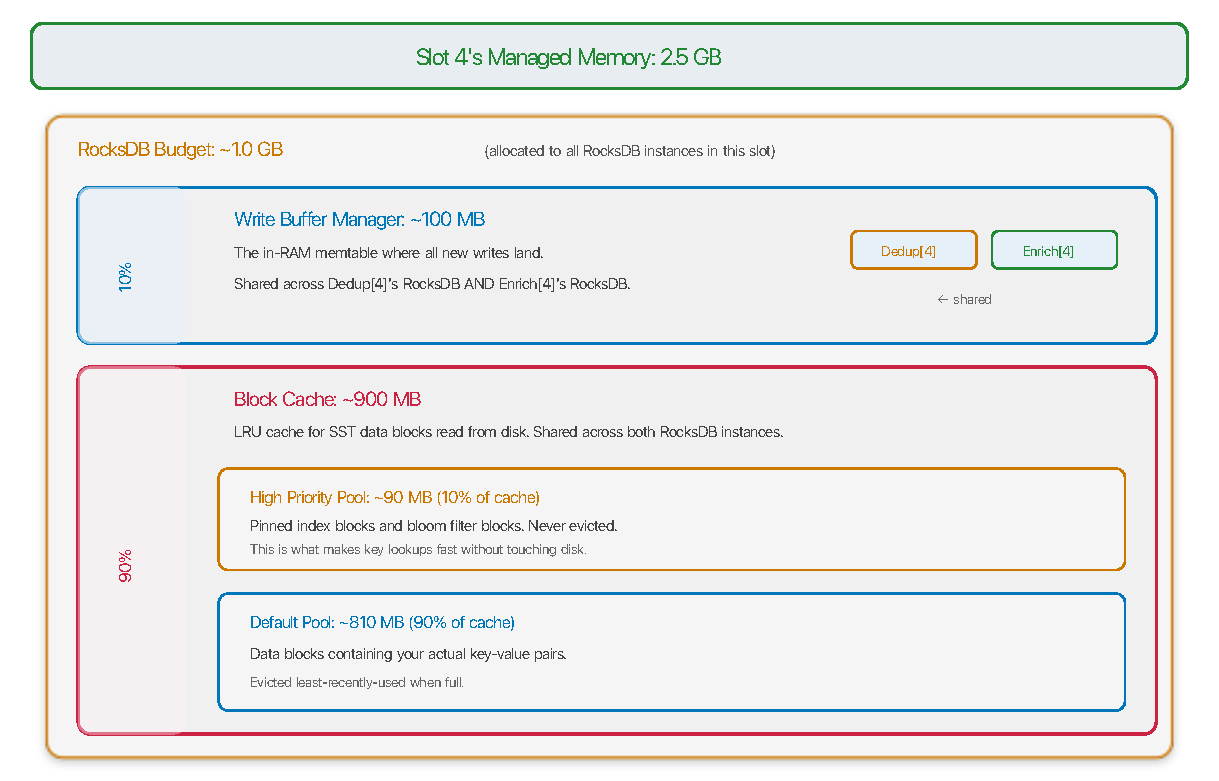
\includegraphics[keepaspectratio, height=0.7\textheight]{fig/slot_memory.pdf}
    \end{figure}

    {\small Dedup[4] and Enrich[4] are separate RocksDB instances but \textbf{share} the block cache within Slot 4. They never compete with Slot 5's RocksDB.}
\end{frame}

\begin{frame}{RocksDB Read Path -- ``Have I Seen This Before?''}
    \begin{figure}[htpb]
        \centering
        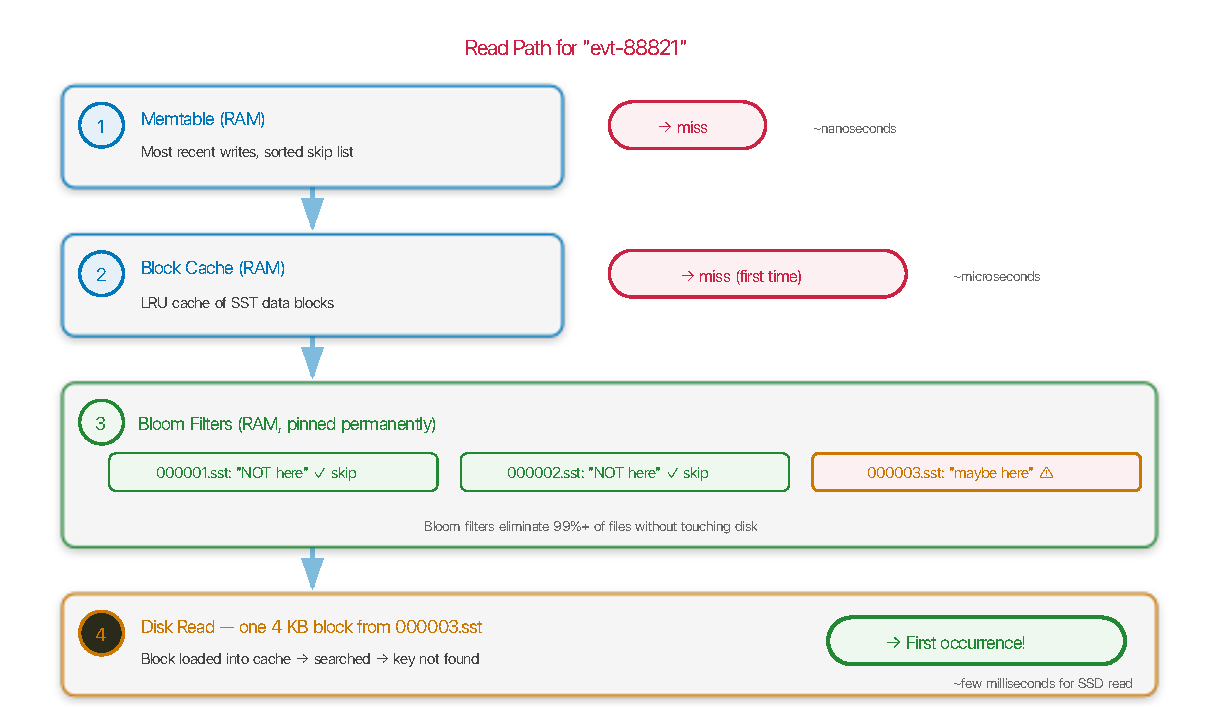
\includegraphics[keepaspectratio, height=0.75\textheight]{fig/rocksdb_read_path.pdf}
    \end{figure}
\end{frame}

\begin{frame}{RocksDB Read Path -- Step by Step}
    \begin{enumerate}
        \item \textbf{Memtable (RAM)} -- most recent writes. Cost: \textbf{nanoseconds}
        \item \textbf{Block cache (RAM)} -- cached 4 KB blocks from SST files. Cost: \textbf{microseconds}
        \item \textbf{Bloom filters (RAM)} -- eliminates 99\%+ of SST files without disk I/O
        \item \textbf{Disk read (SSD)} -- read specific 4 KB block. Cost: \textbf{few milliseconds}
    \end{enumerate}

    \vspace{0.3cm}
    \colorbox{utu_green!20}{\parbox{0.9\textwidth}{
        \centering
        For dedup with short time windows, \textbf{block cache hit rate is 95\%+}. Most lookups are RAM-speed.
    }}
\end{frame}

\begin{frame}{RocksDB Write Path -- Marking ``evt-88821'' as Seen}
    \textbf{Your processing thread never waits on disk:}
    \vspace{0.3cm}

    \begin{enumerate}
        \item Serialize key + value into a \textbf{write batch}
        \item Flush batch into the \textbf{memtable} (a skip list in RAM). Cost: \textbf{microseconds}
        \item Your thread returns immediately. Everything below is background.
    \end{enumerate}

    \vspace{0.3cm}
    \textbf{Background flow (RAM $\rightarrow$ Disk):}
    \begin{enumerate}
        \item Memtable fills up $\rightarrow$ marked \textbf{immutable}; new empty memtable created
        \item Flush thread writes immutable memtable as \textbf{SST file} at Level 0
        \item Compaction threads merge L0 $\rightarrow$ L1 $\rightarrow$ L2 $\rightarrow$ \ldots (each level $\sim$10x larger)
    \end{enumerate}
\end{frame}

\begin{frame}{LSM-Tree: From Memtable to Disk}
    \begin{figure}[htpb]
        \centering
        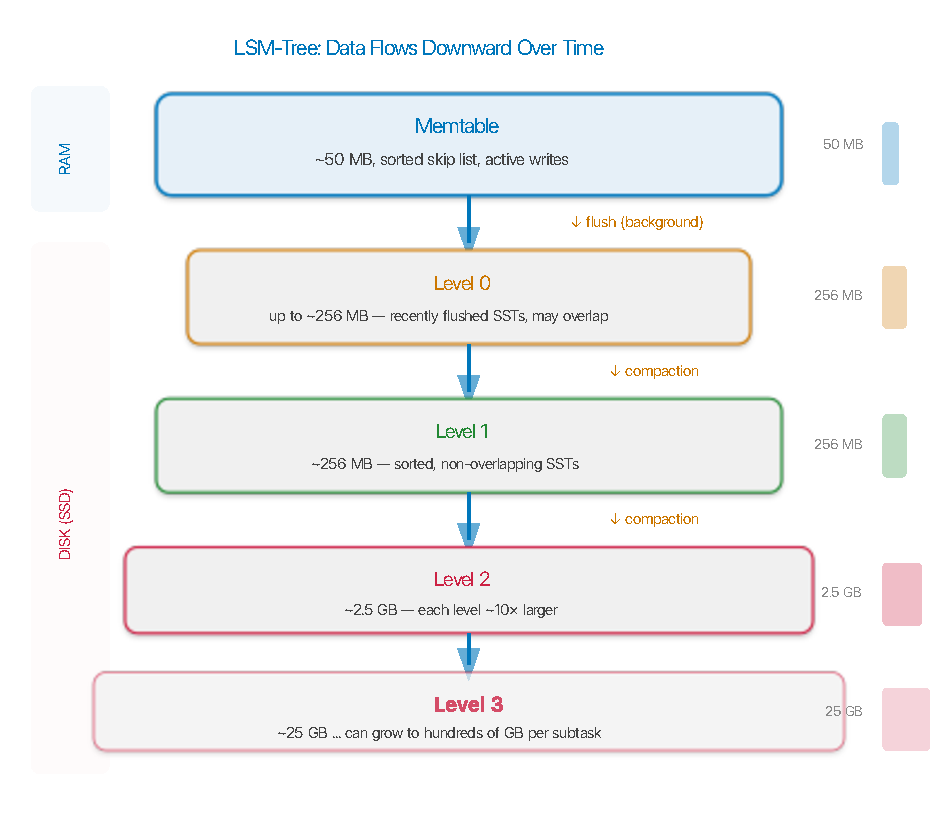
\includegraphics[keepaspectratio, height=0.75\textheight]{fig/lsm_tree.pdf}
    \end{figure}
\end{frame}

\begin{frame}{SST Files on Disk}
    \begin{figure}[htpb]
        \centering
        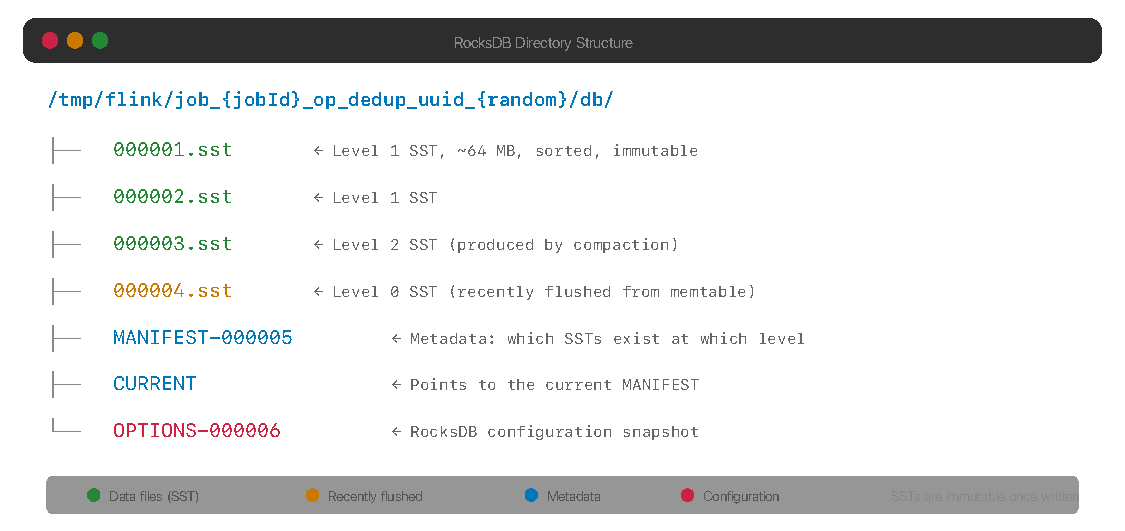
\includegraphics[keepaspectratio, height=0.6\textheight]{fig/rocksdb_directory.pdf}
    \end{figure}

    \vspace{0.2cm}
    \begin{itemize}
        \item Each Flink state descriptor $\rightarrow$ separate \textbf{column family} in RocksDB
        \item SST files are \textbf{immutable} -- never modified after creation
        \item Snapshots = \textbf{hard links} to current SST files (microseconds, any state size)
    \end{itemize}
\end{frame}

% ============================================================
% Enrich & Sink
% ============================================================

\begin{frame}{Chapter 5: The Enrich -- Broadcast State}
    Dedup[4] $\rightarrow$ Enrich[4]: \textbf{same slot, same thread, direct method call} (nanoseconds).

    \vspace{0.3cm}
    \begin{columns}[T]
        \begin{column}{0.48\textwidth}
            \textbf{How Broadcast State Works}
            \begin{itemize}
                \item Keyed state is \textit{partitioned}
                \item Broadcast state is \textbf{replicated}
                \item Every subtask holds the same complete copy
                \item Lives as a \textbf{Java HashMap in JVM heap}
            \end{itemize}
        \end{column}
        \begin{column}{0.48\textwidth}
            \textbf{Write Restriction}
            \begin{itemize}
                \item Processing user events: \textbf{read-only} access
                \item Processing config updates: \textbf{write} access
                \item Why? User events are partitioned; allowing writes would cause 8 copies to diverge
            \end{itemize}
        \end{column}
    \end{columns}
\end{frame}

\begin{frame}{Chapter 6: The Sink -- Writing to Kafka}
    Enrich[4] $\rightarrow$ Sink[4]: also \textbf{chained} -- same slot, same thread.

    \vspace{0.3cm}
    \begin{itemize}
        \item Each Sink subtask has its own \textbf{Kafka producer}
        \item All 8 Sinks write in parallel; Kafka handles concurrent appends natively
        \item JobManager is \textbf{not involved} in data delivery -- only checkpoints and recovery
    \end{itemize}

    \vspace{0.3cm}
    \colorbox{utu_pink!20}{\parbox{0.9\textwidth}{
        \centering
        \textbf{The Kafka transaction is still open.} Records are physically stored but \textbf{invisible} to \texttt{read\_committed} consumers. Our message is in limbo -- written but not committed.
    }}

    \vspace{0.2cm}
    \begin{center}
        It stays this way until the next checkpoint completes.
    \end{center}
\end{frame}

% ============================================================
% Checkpointing & Recovery
% ============================================================

\begin{frame}{Chapter 7: The Checkpoint -- Making It All Durable}
    Every 30s (configurable), the CheckpointCoordinator triggers a distributed snapshot.

    \vspace{0.3cm}
    \textbf{Sink Pre-Commit} (when barrier reaches Sink[4]):
    \begin{enumerate}
        \item \textbf{Flush} all pending records to Kafka broker (transaction still open)
        \item \textbf{Snapshot} producer ID and transaction state to S3
    \end{enumerate}

    \vspace{0.2cm}
    \textbf{Finalization}:
    \begin{enumerate}
        \item All 32 subtasks (8 $\times$ 4 operators) send \texttt{acknowledgeCheckpoint(44)} to JobManager
        \item JobManager writes \texttt{\_metadata} file to S3 -- the \textbf{atomic commit point}
        \item JobManager sends \texttt{notifyCheckpointComplete(44)} to Sinks
        \item Each Sink calls \texttt{commitTransaction()} -- records \textbf{now visible}
    \end{enumerate}
\end{frame}

\begin{frame}{Exactly-Once Achieved}
    \colorbox{utu_green!20}{\parbox{0.95\textwidth}{
        \centering
        \vspace{0.2cm}
        \textbf{Our message is now fully committed:}
        \begin{itemize}
            \item Kafka offset is part of the checkpoint state
            \item Dedup ``seen'' flag is in the RocksDB snapshot on S3
            \item Output record is visible in the output Kafka topic
        \end{itemize}
        \vspace{0.2cm}
        If the entire cluster crashes, Flink restores from S3 and resumes from exactly this point. \textbf{No reprocessing. No duplicates.}
        \vspace{0.2cm}
    }}
\end{frame}

\begin{frame}{When Things Go Wrong -- Pod Crash Recovery}
    TaskManager Pod 3 on Node B gets \textbf{OOM-killed}. Slot 4 \& 5 -- including our Dedup[4] -- are gone.

    \vspace{0.3cm}
    \begin{enumerate}
        \item JobManager detects failure via \textbf{heartbeat timeout}
        \item K8s schedules a \textbf{replacement Pod} (possibly different node)
        \item New TaskManager registers, offers 2 fresh slots
        \item JobManager \textbf{restores from checkpoint 44}: downloads SST files from S3
        \item KafkaSources \textbf{rewind} to checkpointed offsets
        \item KafkaSinks \textbf{abort} uncommitted transactions (zombie fencing)
        \item Processing resumes -- \textbf{brief pause, no data lost, no duplicates}
    \end{enumerate}

    \vspace{0.2cm}
    \colorbox{utu_blue!20}{\parbox{0.9\textwidth}{
        \centering
        K8s handles Pod lifecycle. Flink handles data consistency. Together, the crash is \textbf{invisible}.
    }}
\end{frame}

% ============================================================
\section{Key Takeaways}
% ============================================================

\begin{frame}{Key Takeaways from Flink's Architecture}
    \begin{itemize}
        \item \textbf{Co-locate state with computation}
        \begin{itemize}
            \item Eliminating the network hop is the single biggest performance win
        \end{itemize}

        \vspace{0.15cm}
        \item \textbf{Immutable data structures enable cheap snapshots}
        \begin{itemize}
            \item SST files never modified $\rightarrow$ snapshot = hard links (microseconds)
        \end{itemize}

        \vspace{0.15cm}
        \item \textbf{Barriers over pauses}
        \begin{itemize}
            \item Chandy-Lamport algorithm: coordinate without stopping processing
        \end{itemize}

        \vspace{0.15cm}
        \item \textbf{Incremental over full}
        \begin{itemize}
            \item 500 GB state $\neq$ 500 GB uploaded per checkpoint; only the delta
        \end{itemize}

        \vspace{0.15cm}
        \item \textbf{Two-phase commit for end-to-end exactly-once}
        \begin{itemize}
            \item Sink pre-commits during checkpoint; visible only after finalization
        \end{itemize}
    \end{itemize}
\end{frame}

% ============================================================
\section{Conclusion}
% ============================================================

\begin{frame}{Should You Actually Use Flink?}
    \textbf{The operational commitment is serious:}
    \vspace{0.2cm}

    \begin{columns}[T]
        \begin{column}{0.48\textwidth}
            \begin{itemize}
                \item \textbf{Cluster management}: JobManagers, TaskManagers, S3, monitoring
                \item \textbf{Tuning}: RocksDB memory, network buffers, checkpoint intervals, parallelism
            \end{itemize}
        \end{column}
        \begin{column}{0.48\textwidth}
            \begin{itemize}
                \item \textbf{Upgrades}: Savepoint management, state migration
                \item \textbf{Debugging}: Is it compaction? GC? Network? Key skew?
            \end{itemize}
        \end{column}
    \end{columns}

    \vspace{0.4cm}
    \colorbox{utu_green!20}{\parbox{0.95\textwidth}{
        \centering
        \vspace{0.1cm}
        \textbf{Use Flink when you genuinely need it:}\\
        Millions of msg/s, terabytes of state, exactly-once, event-time processing.\\
        \vspace{0.1cm}
        Under 10K msg/s? A simple consumer with Redis works fine.\\
        Moderate scale + exactly-once? Consider Kafka Streams.
        \vspace{0.1cm}
    }}
\end{frame}

\begin{frame}
    \begin{center}
        {\Huge\calligra Thank You}
    \end{center}
\end{frame}

\end{document}
